\documentclass[12pt]{article} % 12pt 为字号大小 UTF8
\usepackage{amssymb,amsfonts,amsmath,amsthm}
%\usepackage{fontspec,xltxtra,xunicode}
%\usepackage{times}

%----------
% 定义中文环境
%----------

\usepackage{xeCJK}

% \setCJKmainfont[BoldFont={SimHei},ItalicFont={KaiTi}]{SimSun}
% \setCJKsansfont{SimHei}
% \setCJKfamilyfont{zhsong}{SimSun}
% \setCJKfamilyfont{zhhei}{SimHei}

% \newcommand*{\songti}{\CJKfamily{zhsong}} % 宋体
% \newcommand*{\heiti}{\CJKfamily{zhhei}}   % 黑体


%----------
% 版面设置
%----------
%首段缩进
\usepackage{indentfirst}
\setlength{\parindent}{2.1em}

%行距
\renewcommand{\baselinestretch}{1.2} % 1.4倍行距

%页边距
\usepackage[a4paper]{geometry}
\geometry{verbose,
  tmargin=3cm,% 上边距
  bmargin=3cm,% 下边距
  lmargin=3cm,% 左边距
  rmargin=3cm % 右边距
}


%----------
% 其他宏包
%----------
%图形相关
\usepackage[x11names]{xcolor} % must before tikz, x11names defines RoyalBlue3
\usepackage{graphicx}
\usepackage{pstricks,pst-plot,pst-eps}
\usepackage{subfig}
\def\pgfsysdriver{pgfsys-dvipdfmx.def} % put before tikz
\usepackage{tikz}

%原文照排
\usepackage{verbatim}

%网址
\usepackage{url}

%----------
% 习题与解答环境
%----------
%习题环境
\theoremstyle{definition} 
\newtheorem{exs}{习题}

%解答环境
\ifx\proof\undefined\
\newenvironment{proof}[1][\protect\proofname]{\par
\normalfont\topsep6\p@\@plus6\p@\relax
\trivlist
\itemindent\parindent
\item[\hskip\labelsep
\scshape
#1]\ignorespaces
}{%
\endtrivlist\@endpefalse
}
\fi
\renewcommand{\proofname}{\it{证明}}

% \begin{exs}
% 请证明勾股定理。
% \end{exs}
% \begin{proof}
% 这是证明。末尾后会自动添加方块以示结束。
% \end{proof}

%----------
% 我的自定义
%----------

\newcommand{\horrule}[1]{\rule[0.5ex]{\linewidth}{#1}} 	% Horizontal rule

\renewcommand{\refname}{参考文献}
\renewcommand{\abstractname}{\large \bf 摘\quad 要}
\renewcommand{\contentsname}{目录}
\renewcommand{\tablename}{表}
\renewcommand{\figurename}{图}

\setlength{\parskip}{0.4ex} % 段落间距

\usepackage{enumitem}
\setenumerate[1]{itemsep=0pt,partopsep=0pt,parsep=\parskip,topsep=5pt}
\setitemize[1]{itemsep=0.4ex,partopsep=0.4ex,parsep=\parskip,topsep=0.4ex}
\setdescription{itemsep=0pt,partopsep=0pt,parsep=\parskip,topsep=5pt}


%==========
% 正文部分
%==========

\begin{document}

\title{
{\normalfont\normalsize\textsc{
Peking University\\
Computer Architectures, Spring 2024 \\[25pt]}}
\horrule{0.5pt}\\
\sffamily{“冯·诺依曼计算机结构”\\读书报告}
\horrule{1.8pt}\\[20pt]
}
\author{梁昱桐\quad 2100013116\\lyt0112@outlook.com}
% \date{} % 若不需要自动插入日期,则去掉前面的注释;{ } 中也可以自定义日期格式

\begin{titlepage}
\maketitle
\vspace{30pt}

% \begin{abstract}
% \normalsize \ \ 这是中文摘要。大概写满这一页可以了。摘要又称概要、内容提要。摘要是以提供文献内容梗概为目的,不加评论和补充解释,简明、确切地记述文献重要内容的短文。其基本要素包括研究目的、方法、结果和结论。具体地讲就是研究工作的主要对象和范围,采用的手段和方法,得出的结果和重要的结论,有时也包括具有情报价值的其它重要的信息。\\[5pt]
% \indent \ \ \textbf{关键词}:图卷积神经网络,复杂网络,表示学习
% \end{abstract}

\thispagestyle{empty}
\end{titlepage}

\tableofcontents
\thispagestyle{empty}

\newpage
\setcounter{page}{1}

\section{摘要}

本篇读书报告所读的主要文献:《EDVAC报告书的第一份草案》(First Draft of a Report on the EDVAC)是著名美籍计算机科学家冯诺依曼所撰写并于1945年6月30日发表的。
在这份报告中,作者描述了使用“存储程序逻辑设计”的新型运算设备,这一概念被后世的电脑设备广泛使用,此种设计架构也被称为“冯诺依曼架构”。\cite{vonNeumann1945edvac}

\subsection{DEFINITIONS}

本节介绍了高速自动数字计算系统的基本概念和结构,强调了自动计算系统能够执行复杂计算的能力,必须接收详细的指令,并能够自动执行这些指令并记录结果。
同时,也提到了设备可能发生的故障及其可能的自动识别和修正机制。

\subsection{MAIN SUBDIVISIONS OF THE SYSTEM}

本节讨论了高速自动计算设备的五个关键组成部分:中央算术部件(CA)、中央控制(CC)、存储器(M)、输入设备(I)和输出设备(O)。
它强调了设备为高效执行算术运算、逻辑控制和长复杂操作序列所需的存储能力,以及与外部媒介交换数据的能力。
此外,还探讨了内部存储器(M)与外部存储媒介(R)之间的区别和互补性,以及为何内部存储对于设备的高速和高效运行至关重要。

\subsection{PROCEDURE OF DISCUSSION}

本节是承上启下的一节,由于细分环节已经结束,接下来就会对各个部分
进行细致的讨论。
这里提出了具体分析时需要遵从的一些原则:五个部分彼此依
赖,不可独立讨论;需要注意故障检测、定位以及纠正的工作,也即需要重视各
部分中检查并修正错误的装置。

\subsection{ELEMENTS, SYNCHRONISM NEURON ANALOGY}

本节探讨了数字计算设备中使用的基本元素及其工作原理,其中强调了这些元素如继电器一样具有离散平衡状态的特性。
这些元素能够在没有外部支持的情况下保持在特定的状态中,或者依赖外部刺激来维持其状态。

进一步讨论了数字计算设备的计时方式,即是通过内部元素的连续反应时间自主计时,还是依赖于外部时钟来计时,从而定义了同步与异步设备的概念。
此外,文章指出了高等动物的神经元在功能上与讨论的计算元素具有相似性,尤其是在兴奋和传递刺激方面,同时也提到了通过电报继电器或真空管模拟简化的神经元功能的可能性。

\subsection{PRINCIPLES GOVERNING THE ARITHMETICAL OPERATIONS}

本节主要从中央算数部分(CA)的角度出发,讲述了控制算术运算的原则。

围绕了计算机早期设计的关键概念,特别是使用真空管作为逻辑门和触发器,以及二进制系统的选择和应用。
真空管的使用基于其全或无的特性,使得设备能够通过电子脉冲在不同的稳定状态之间切换,从而实现逻辑运算。
这些触发电路的设计简化了数字处理,尤其是在进行算术运算时。文中强调了二进制系统在简化乘法和除法运算方面的优势,因其避免了十进制系统中复杂的步骤和计算表的使用。

在讨论到计算机的运算速度和效率时,非真空管设备由于元件的反应时间较长,需要采用一系列加速和“望远镜式”操作来提高效率。
然而,这种方法虽然能够减少运算时间,但却以增加设备复杂度和元件数量为代价。与之相反,真空管设备因其极短的反应时间(微秒级),
使得即使是未经优化的操作也能接受,从而提出了一种简化设备以减少元件数量和提高可靠性的设计理念。

\subsection{E-ELEMENTS}

本节基于上一节,继续讨论中央算数部分 (CA)的处理方法,引入更具体和技术性的细节。

为了方便讨论,使用了一个假想的元素来代替真实的真空管元件,这个假想元素被称为E元素,它能够接收兴奋性和抑制性刺激,并在一定的延迟后发出信号。
E元素的设计旨在模拟人类神经元的功能,其特点包括固定的突触延迟时间τ,以及能够通过电子管电路实现的不同阈值和延迟变体。

此外,本节还讨论了E元素网络与真空管实现之间的对比,指出每个E元素通常需要1-2个真空管来实现,这包括了放大和脉冲整形的需求,但不包括电源供应。

\subsection{CIRCUITS FOR THE ARITHMETICAL OPERATIONS +, ×}

本节详细介绍了计算设备中用于执行加法和乘法运算的电路设计。加法器网络能够处理二进制加法并输出结果,而乘法器网络则需要内置记忆功能,以便在乘法过程中暂存乘数和被乘数。
乘法过程包括一个辅助网络和一个阀门网络,控制被乘数是否加到部分乘积总和中。

出于“将多个事件置于时间连续中,而不是空间并置中”这样的设计思想,作者团队构造出同时进行 30 位计算的运算器。

此外,还讨论了乘法器网络的时间控制和延迟处理,但未涉及数字的符号和二进制点位置处理,这些问题预计在后续讨论中解决。

\subsection{CIRCUITS FOR THE ARITHMETICAL OPERATIONS −, ÷}

本节讨论了在二进制计算系统中实现减法和除法运算的电路设计,
深入探讨了在二进制计算系统中实现基本算术运算的电路设计,包括减法和除法,强调了符号位和二进制点的处理方法以及利用补码实现减法的技术。

首先,介绍了如何通过为二进制数引入符号位和二进制点来处理正负数和小数。
在这种约定下,最左侧的位用作符号位,0表示正数,1表示负数。接着,详细说明了如何通过使用加法器来构建减法器网络,方法是将被减数的每一位取补后加上1,
即实现二进制的一种补码运算。此外,还介绍了构建除法器网络的方法,该方法通过连续从被除数中减去除数并根据结果的正负决定商的相应位是0还是1,以实现二进制除法运算。

\subsection{THE BINARY POINT}

本节讨论了二进制小数点的设置对乘法和除法运算的重要性。明确了所有参与计算的数必须是非负数的前提下,探讨了二进制小数点位置如何影响乘积的计算和表示。
特别指出,当进行乘法运算时,如果两个因数的二进制小数点位置分别在第i和第j位,则乘积的二进制小数点位置应在第\(k = i + j - 1\)位。此外,
为了确保所有数字在计算过程中始终位于-1与1之间,提出了在计算前通过适当调整数字(乘以2的负幂)来保证这一条件。
最后,讨论了四舍五入的必要性和方法,提出了一种简单的四舍五入规则,以及实现这一规则的装置。

\subsection{CIRCUIT FOR THE ARITHMETICAL OPERATION √ OTHER OPERATIONS}

本节讨论了在计算机体系结构(CA)中实现平方根(√)运算的方法,以及是否将它和其他算术运算(如加法、减法、乘法和除法)纳入CA的考虑。

平方根运算与除法运算极为相似,通过对部分余数执行双位左移和减法操作来逐步构建平方根。这一过程不需要额外的硬件支持,只需简单的逻辑调整即可。此外,讨论还涵盖了将乘法、除法和平方根运算简化为加法的可能性,以及为什么直接算术方法更为合理。

最终,文中建议将加法、减法、乘法、除法和平方根运算作为基本操作包含在CA中,因为它们具有相似的操作复杂度和时间消耗,而尝试用函数表或迭代方法替代这些操作会增加逻辑控制的复杂性和执行时间。

\subsection{ORGANIZATION OF CA. COMPLETE LIST OF OPERATIONS}

本节概述了CA(计算装置)的组织结构和操作列表。CA主要被组织为一个分频器,通过适当的控制来满足其他操作的需求。

重点讨论了CA与M(存储单元)之间的传输连接,强调了能够从M的任何部分向CA传输数据的重要性,并提出了通过时间序列而非空间并置来简化连接的方法。

最后,列出了CA必须能够执行的十项操作:加、减、乘、除、开平方、直接传输i、j,判断符号s,以及二进制与十进制之间的转换操作db和bd。
这一讨论为进一步探讨CA的控制问题和特定网络操作铺平了道路。

\subsection{CAPACITY OF THE MEMORY M. GENERAL PRINCIPLES}

本节讨论了计算机存储系统的设计和容量需求评估。

作者首先介绍了存储器的分类和对应的容量需求,包括操作指令、函数表、初始值和中间值等。接着,文中探讨了利用延迟元件(如线性电路和非线性电路)
构建存储器的可能性,并详细分析了不同类型的存储器(如延迟存储器和图标管存储器)的特点和潜在优势。

最后,作者总结了存储器的总容量、单个存储器元件的容量以及构建高效存储系统所需的技术挑战和解决方案。

\subsection{ORGANIZATION OF M}

本节讨论了基于延迟存储器的组织结构,包括其终端器官A(放大器)和SG(开关门控器官)的设计和功能。
SG的主要功能是在特定时刻建立或断开与其它设备部分(如CC、CA等)的连接,以实现信息的传输或循环。
通过引入E元素构建SG,进一步讨论了SG在不同状态下(即SG开启或关闭状态)的连接方式及其通过Lo和Li线与其它部分的连接。
此外,还介绍了SG的E网络设计,以及为实现SG不同状态下的功能而在CC中设置的补充连接。
最后,讨论了如何通过CC中的特定线路激活SG,以及如何表示和处理要激活的SG的编号。

\subsection{CC AND M}

本节分析中央控制中心(CC)的工作原理,特别是如何解析和执行来自存储模块(M)的指令。
CC的功能包括接收指令、解释指令以及执行或触发相应的操作。因此,我们首先需要列举和定义控制设备的指令系统,即描述设备使用的代码及其数学、逻辑意义和操作重要性。

指令分四类:
\begin{enumerate}
  \item 指示计算单元(CA)执行特定操作的指令
  \item 数据在不同位置间的转移指令
  \item 改变CC与M连接点的指令,以从新位置获取下一条指令
  \item 控制输入输出设备的操作指令
\end{enumerate}

此外,我们还讨论了转移指令的两种类型:短暂转移和永久转移,以及在进行数据或指令转移时需要等待的时间问题。
最后,提出了对DLA和小周期的编号方法,以及在不同情况下小周期编号如何变化的细节。

\subsection{THE CODE}

本节提供了对M中内容完整分类的基础,通过一系列连续的二分法给出了这一分类。此分类使我们能够制定出控制CC(因而控制整个设备)的逻辑代码。M的内容是由存储单元组成,每个单元通过存在或缺失刺激来表示二进制数字1或0。这些单元被组织成32单元的小周期,这些小周期在我们将要介绍的代码中将直接具有意义。小周期分为标准数字和指令两类,通过其第一个单元的值(即i0为0表示标准数字,为1表示指令)来区分。

最后,根据以上讨论制定代码,描述每种可能的小周期的类型、含义、简短符号和代码符号。

\section{冯诺依曼结构特点分析}

冯诺依曼计算机结构的主要特点总结如下\cite{vonNeumann1945edvac}:

\begin{enumerate}
  \item \textbf{存储程序控制}:冯诺依曼结构的核心特点之一是使用存储程序逻辑设计,即程序指令和数据统一存储在计算机的内存中。这种设计使得计算机能够自动、顺序地执行存储在内存中的指令序列,极大地提高了计算机的灵活性和效率。
  \item \textbf{五大组成部分}:冯诺依曼结构由五个主要部分组成,分别是中央算术部件(CA)、中央控制(CC)、存储器(M)、输入(I)和输出(O)。这五部分构成了一个完整的计算系统,可以高效执行算术运算、逻辑控制和复杂操作序列。
  \item \textbf{二进制系统}:在冯诺依曼结构中,采用二进制表示数据和指令。二进制系统简化了计算机的设计,特别是在进行算术运算(如加法、减法、乘法和除法)时,二进制的使用使得硬件实现更为简单和高效。
  \item \textbf{同步设备}:冯诺依曼体系结构强调了同步设备的概念,即计算机的各个部分在一个统一的时钟信号下工作,保证了操作的准确性和稳定性。这种同步机制使得计算机能够以一定的速率稳定运行。
  \item \textbf{内部和外部存储的区别}:冯诺依曼结构明确区分了内部存储器(M)和外部存储媒介(R),并强调了内部存储对于设备的高速和高效运行至关重要。内部存储器用于存储当前正在执行的程序和数据,而外部存储用于长期存储数据和程序。
  \item \textbf{错误检测和纠正}:在冯诺依曼结构中,也考虑了设备可能发生的故障及其自动识别和修正机制。这表明了早期计算机设计已经开始关注系统的可靠性和稳定性。
  \item \textbf{基本算术运算电路设计}:冯诺依曼结构详细讨论了如何通过电子电路实现基本的算术运算,如加法、减法、乘法、除法和开平方等。这些运算的电路设计是构建高效计算机系统的基础。
  \item \textbf{模块化和组织结构}:冯诺依曼结构通过模块化的设计理念,明确了计算机各个部件的功能和相互之间的联系。这种组织结构不仅有助于理解计算机的工作原理,也为后续计算机的发展提供了一个坚实的基础。
\end{enumerate}

\section{当前计算设备分析对比}

我目前使用的计算设备是苹果公司于 2021 年推出的 MacBook Pro\cite{MacBookPro2023},配备了 M1 Pro 处理器。
这款设备的设计基于苹果自研的 ARM 架构,与传统的冯诺依曼架构相比,它在处理效率和能耗控制上都有显著的提升。

\begin{figure}[h]
  \centering
  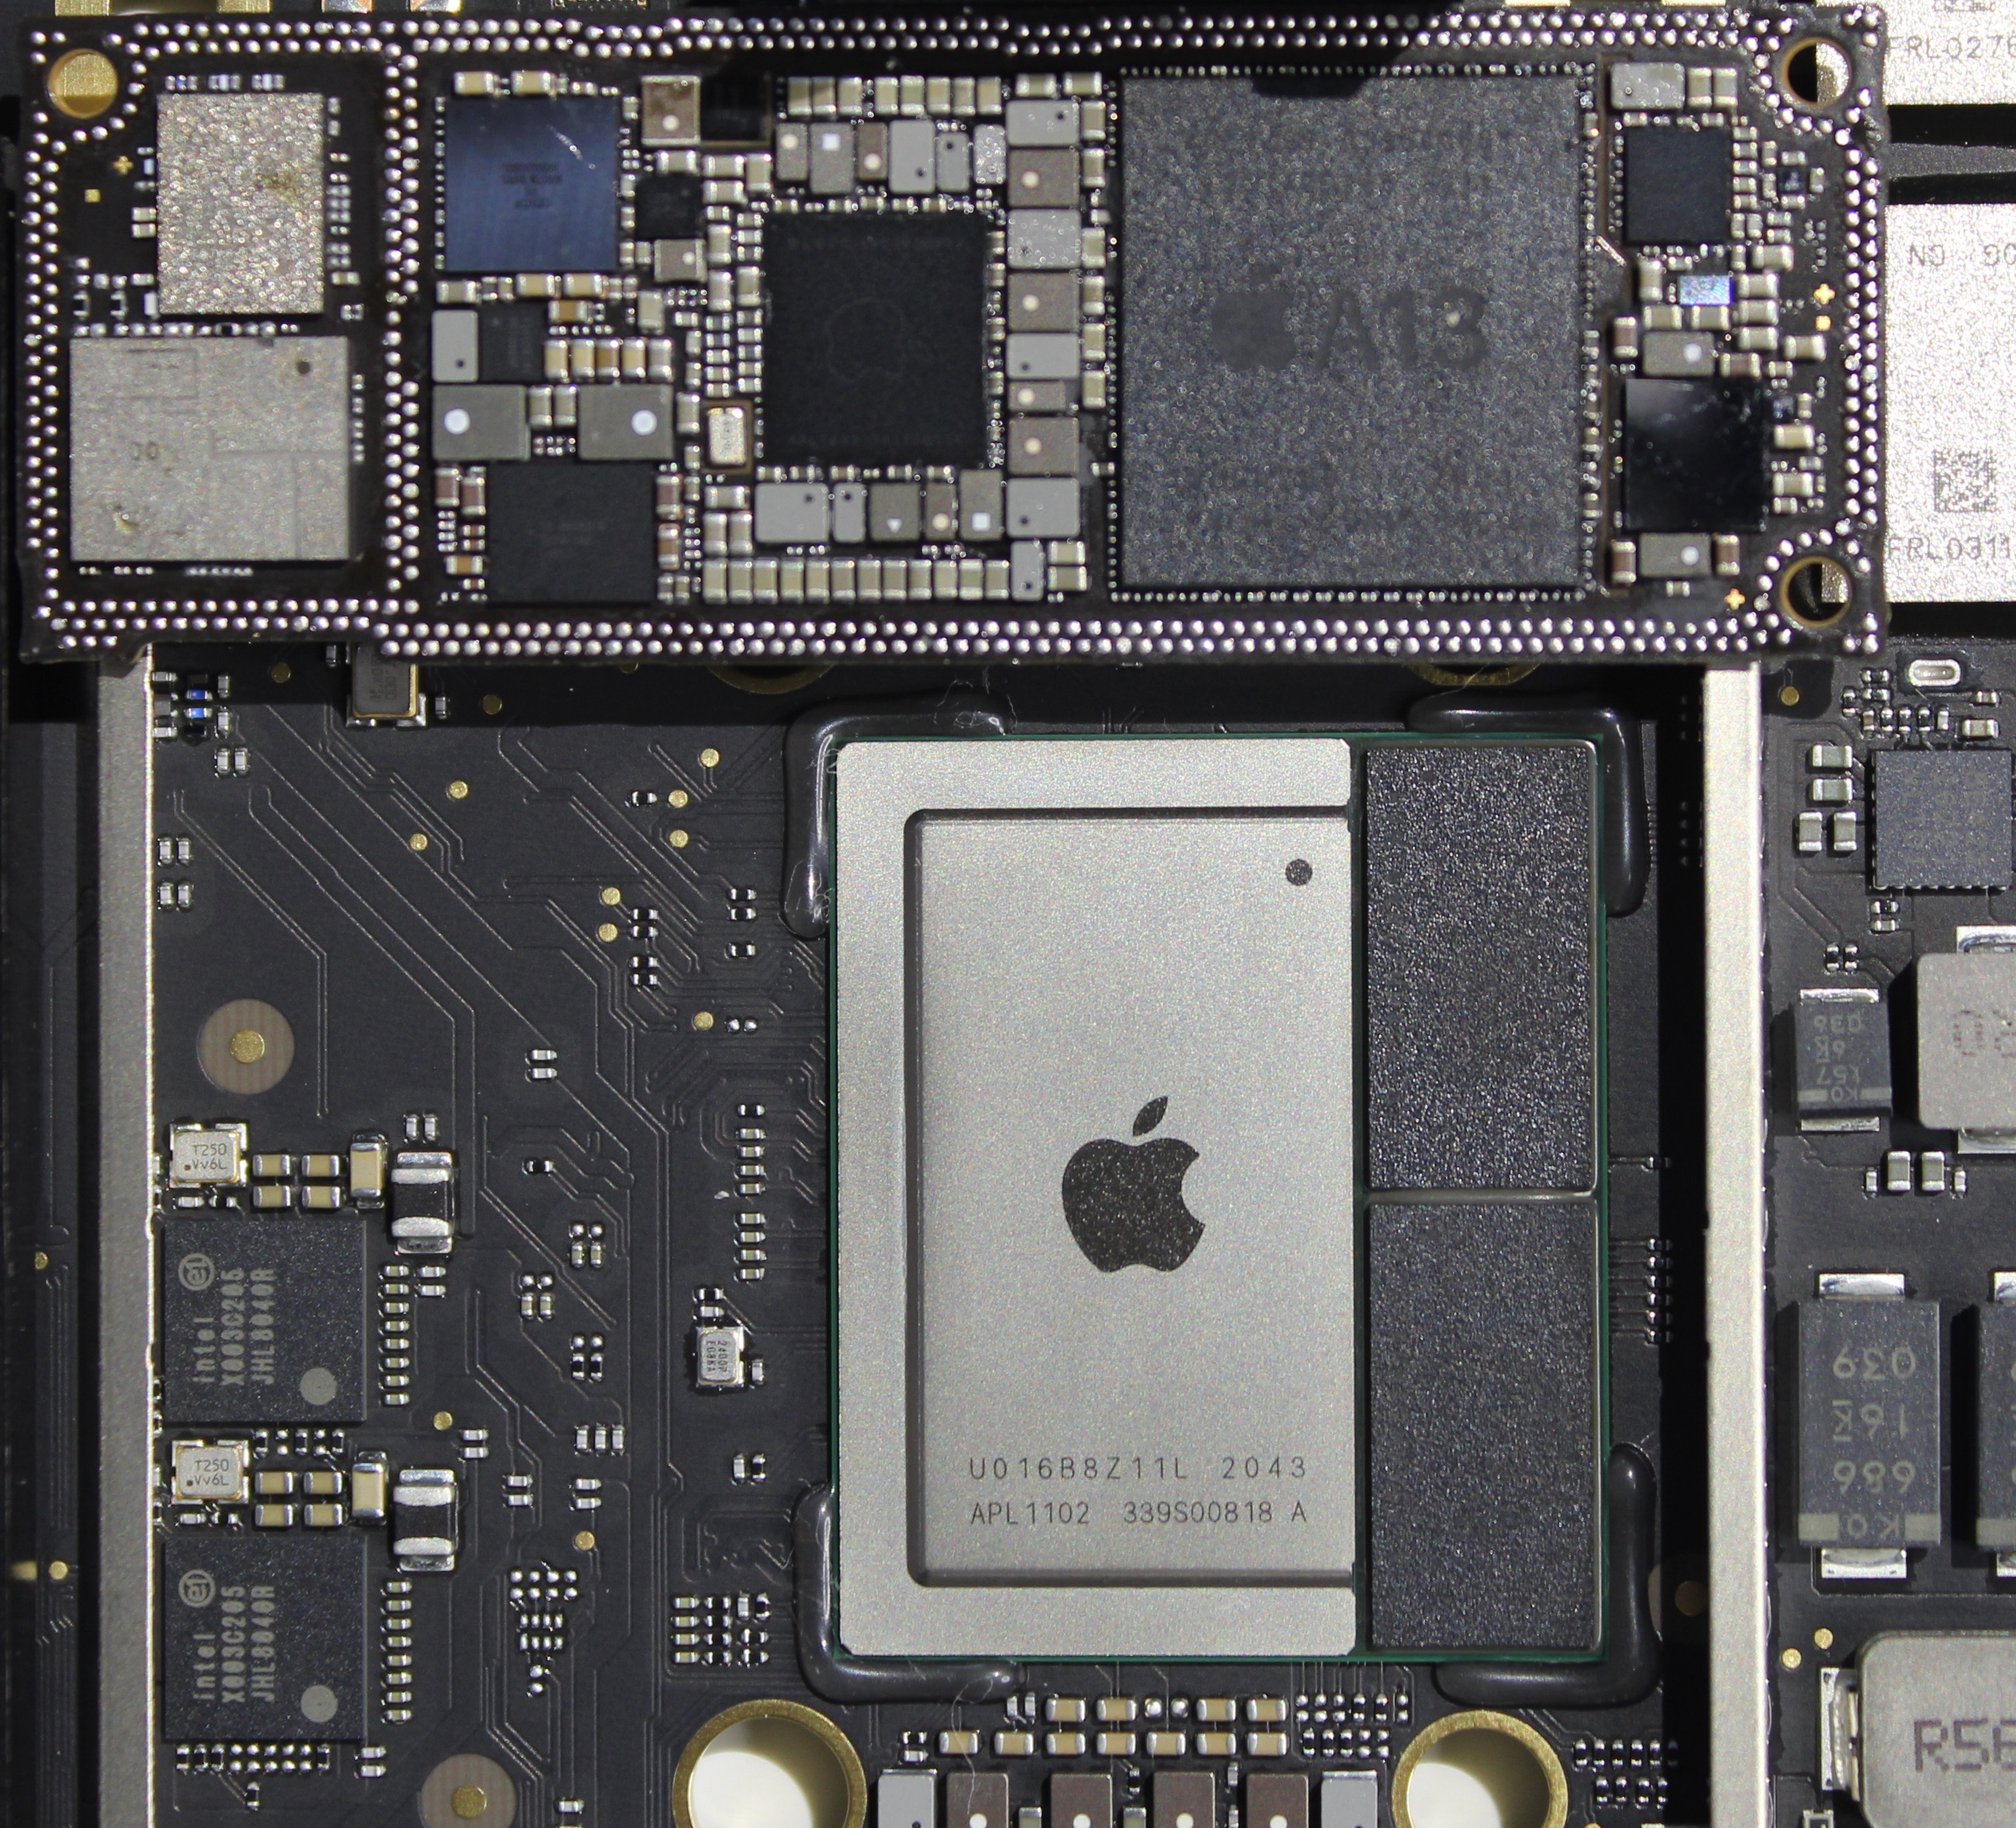
\includegraphics[width=0.6\textwidth]{./figs/M1_A13_comparison_MacMini9_1_M1.jpg}
  \caption{M1 Chip\cite{Sonic84002020Image}}
  \label{fig:AppleM1}
\end{figure}

具体来说,M1 Pro 处理器\cite{AppleM12023}的构成如下:

\begin{enumerate}
  \item \textbf{中央处理架构}:M1 Pro 搭载了高性能和高效能的 CPU 核心,采用了 Apple 的“Firestorm”和“Icestorm”技术。它包含 8 个高性能核心和 2 个高效能核心\cite{GSMArenaAppleM1},通过使用大.LITTLE 技术,能够根据不同的工作负载智能切换,以优化能源使用效率。
  \item \textbf{中央控制架构}:M1 Pro 基于 Apple 自研的 ARMv8.5-A 指令集,这一指令集的设计使得 M1 Pro 在执行各类应用程序时,能够提供更快的处理速度和更高的能效比。
  \item \textbf{存储器架构}:M1 Pro 采用了统一内存架构,内存与处理器集成在同一芯片上,能够实现高带宽、低延迟的数据访问。这种设计不仅提升了性能,还降低了功耗。
  \item \textbf{输入输出设备}:MacBook Pro 配备了多种输入输出接口,包括三个 Thunderbolt 端口、一个 HDMI 端口、SD卡读卡器以及 MagSafe 充电接口等。这些丰富的接口设计极大地提升了设备的扩展性和便携性。
\end{enumerate}

综上所述,M1 Pro 搭载的 MacBook Pro 相较于传统基于 x86 架构的个人计算机,在处理效率、能源使用和系统集成度上都有显著的改进。
特别是它的高效能 CPU 核心和统一内存架构,使得在执行复杂计算任务时,能够展现出卓越的性能。
同时,多样化的输入输出接口满足了对于高速数据传输和多显示器输出的需求。

\section{“非冯结构”调研分析}

非冯·诺伊曼架构主要包括哈佛架构、改进的哈佛架构、数据流架构和神经网络架构等\cite{Siriwardhane2020ComputerArchitecture}。
这些架构相对于传统的冯·诺伊曼架构,在某些特定的应用场景下展现出了显著的优势。

\subsection{哈佛架构}

哈佛架构是一种将程序指令存储和数据存储分开的存储器结构。这种架构的主要特点是使用两个独立的存储器模块来分别存储指令和数据,
并且每个存储模块都有自己的访问总线,使得数据和指令的读取可以并行进行,从而提高了数据吞吐量和运算速度\cite{HarvardArchitecture, Pawson2022MythHarvard}。

\begin{figure}[h]
  \centering
  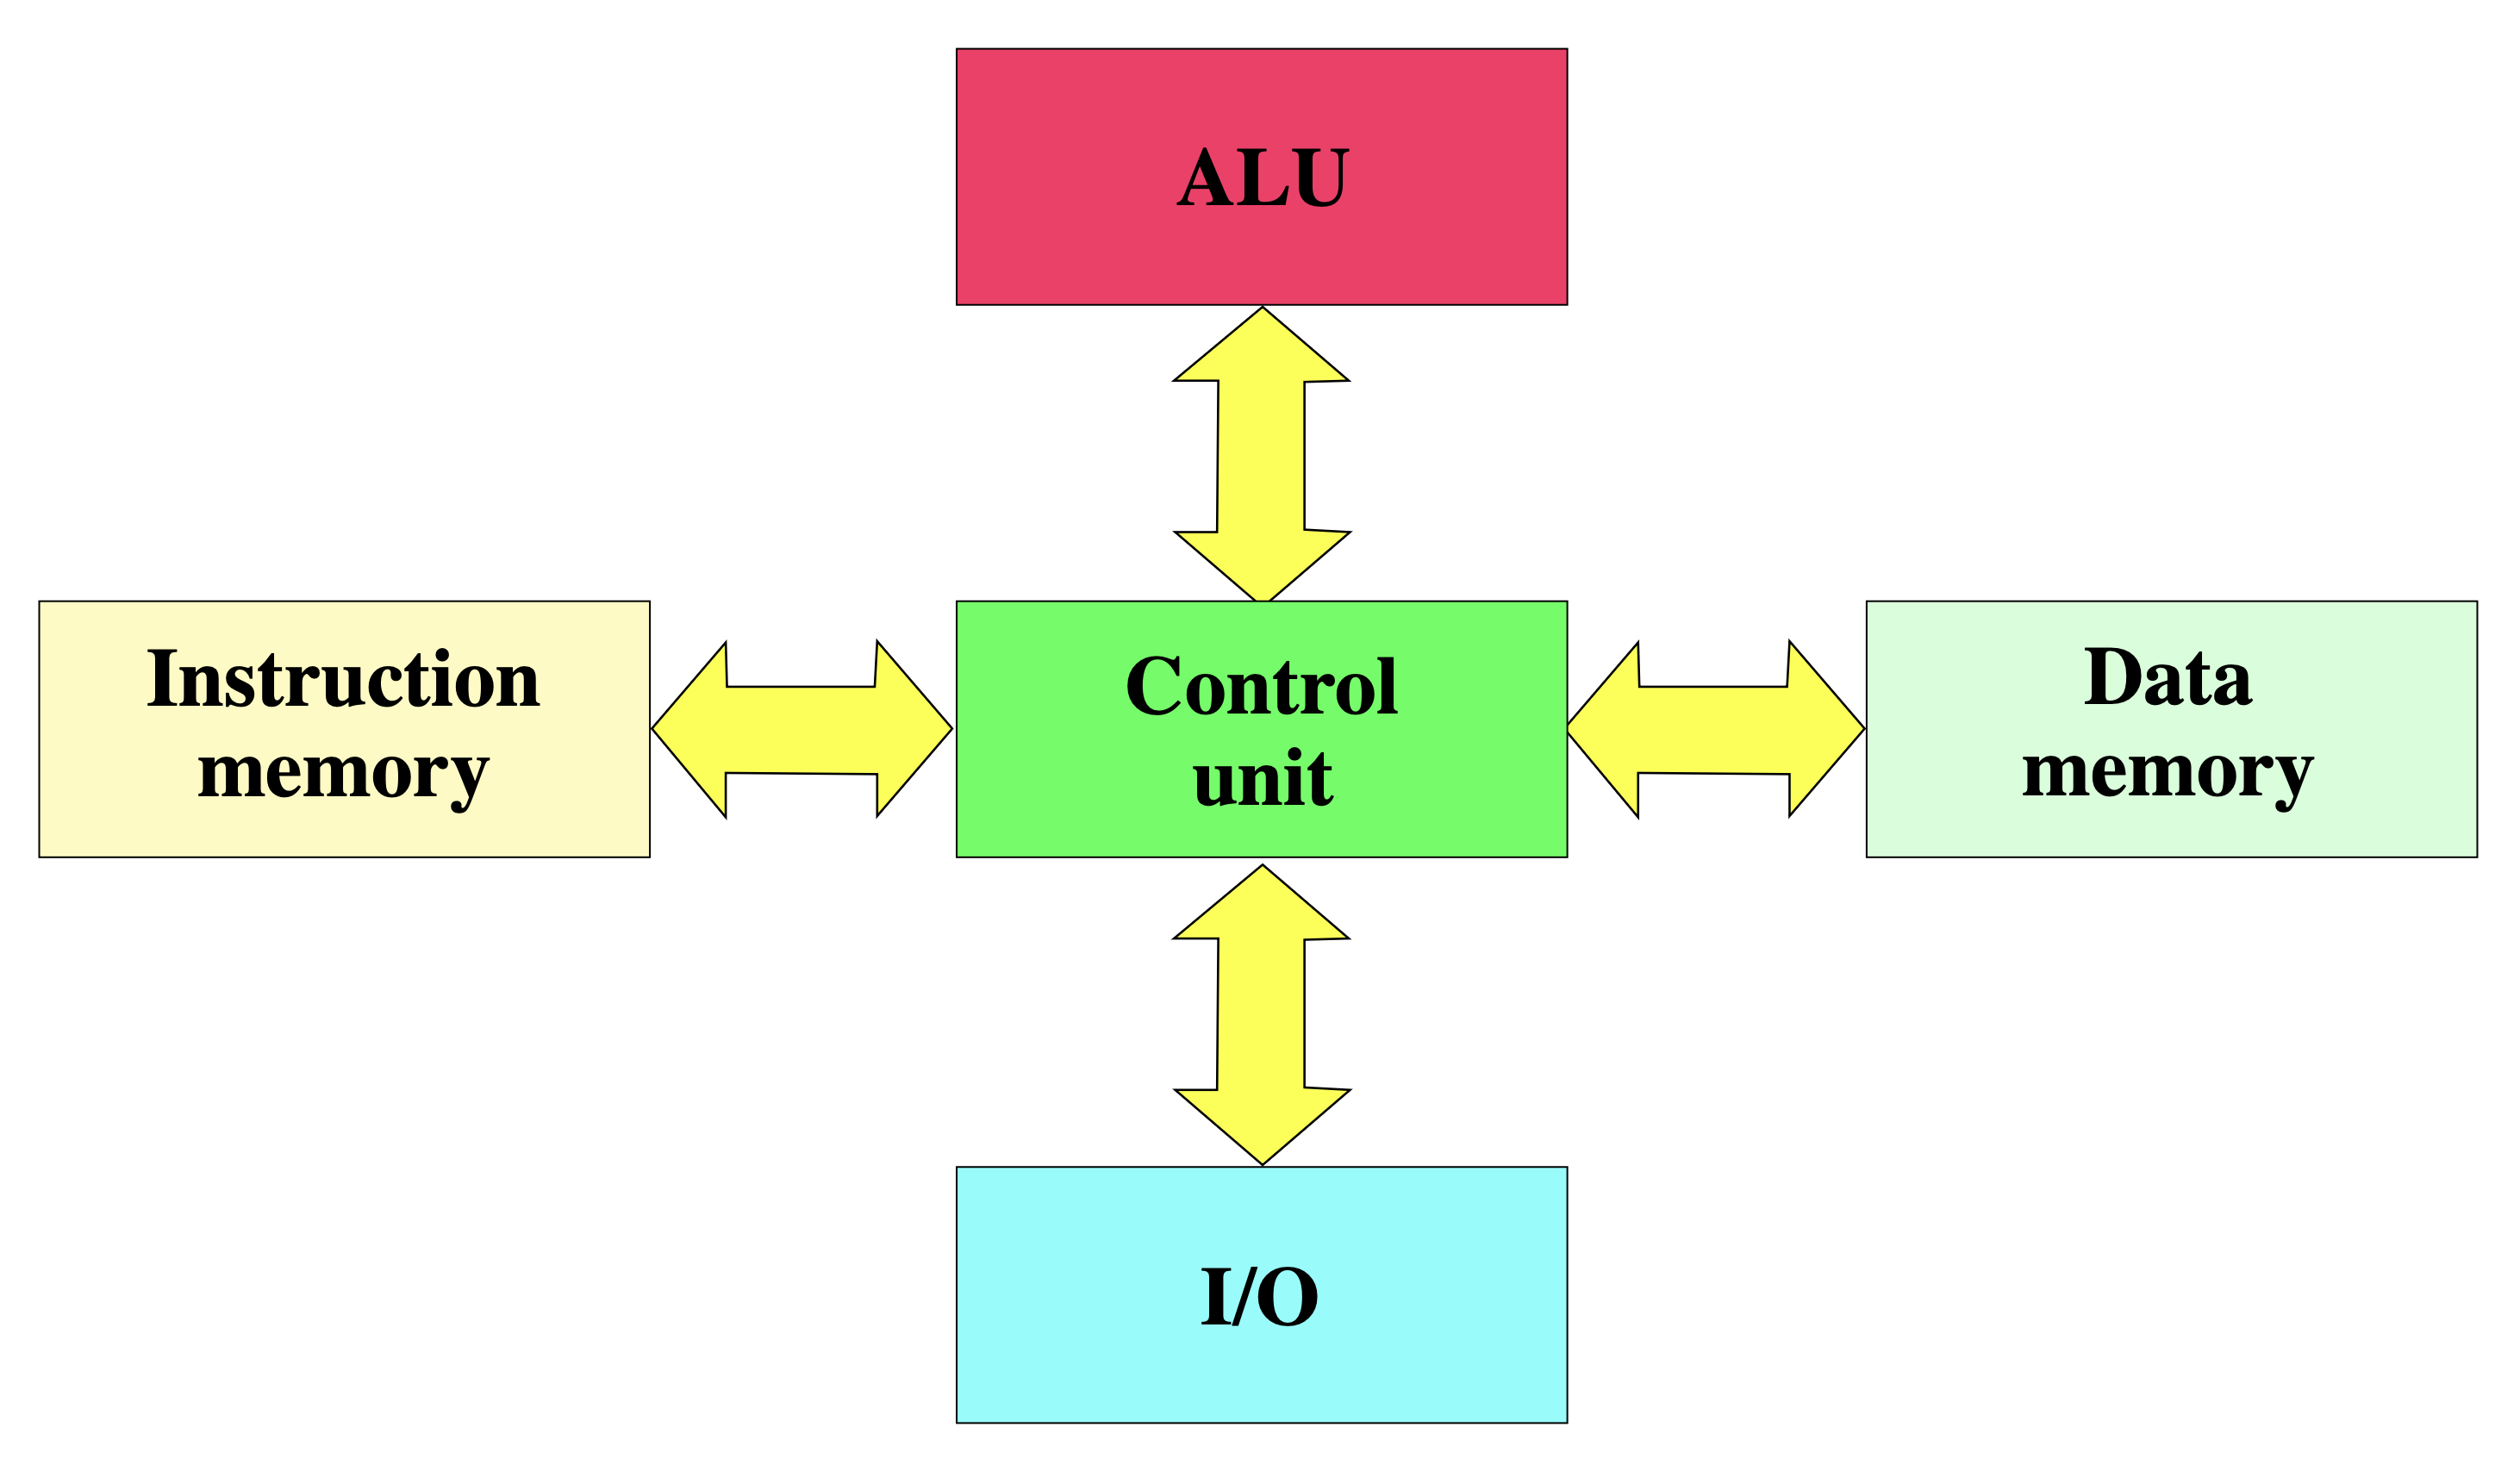
\includegraphics[width=0.6\textwidth]{./figs/Harvard_architecture.png}
  \caption{哈佛架构示意图\cite{HarvardArchitecture}}
  \label{fig:harvard-architecture}
\end{figure}

\textbf{优点:}
\begin{enumerate}
  \item \textbf{并行处理能力}:由于指令和数据分别存储,并且有独立的访问路径,因此可以同时访问指令和数据,提高了处理速度。
  \item \textbf{安全性}:指令和数据的物理隔离也增加了系统的安全性,防止了数据泄露和指令篡改。
\end{enumerate}

\textbf{缺点:}
\begin{enumerate}
  \item \textbf{硬件成本}:由于需要额外的存储器模块和访问总线,使得系统的硬件成本增加。
  \item \textbf{灵活性较差}:由于指令和数据分开存储,因此对于需要频繁修改指令的应用场景不太适用。
\end{enumerate}

\subsection{改进的哈佛架构}

改进的哈佛架构在哈佛架构的基础上做了一些松绑,允许一定程度上的指令和数据之间的交互,同时保持了哈佛架构的并行处理能力。这种架构常见于现代微处理器中,如ARM、x86等\cite{HarvardArchitecture, Pawson2022MythHarvard}。

\textbf{优点:}
\begin{enumerate}
  \item \textbf{并行处理能力}:改进的哈佛架构保留了哈佛架构的并行处理能力,能够提高系统的运算速度。
  \item \textbf{灵活性}:相比于哈佛架构,改进的哈佛架构允许指令和数据之间的交互,使得系统更加灵活,适用于更多的应用场景。
\end{enumerate}

\textbf{缺点:}
\begin{enumerate}
  \item \textbf{复杂性}:相比于哈佛架构,改进的哈佛架构需要更多的硬件支持,使得系统的复杂性增加。
\end{enumerate}

\subsection{数据流架构和神经网络架构}

数据流架构和神经网络架构是另外两种非冯·诺伊曼架构,它们主要针对特定类型的算法和处理需求进行了优化\cite{Siriwardhane2020ComputerArchitecture}。

\textbf{数据流架构:}主要优点在于能够根据数据的准备情况动态地执行指令,非常适合并行计算和流处理任务。

\textbf{神经网络架构:}则是专为模拟人工神经网络而设计,对于深度学习和人工智能任务具有天然的优势。

\section{补充信息}

冯诺依曼架构是一个非常经典的计算机体系结构,如今仍活跃在我们身边。

然而,随着计算机技术的不断进步,冯·诺依曼架构的局限性也逐渐显现:

\begin{enumerate}
  \item \textbf{内存瓶颈}:由于计算机的内存和处理器之间的数据传输速度有限,导致了内存瓶颈,使得计算机的处理能力受到限制。这也是冯·诺依曼架构的一个重要局限性。
  \item \textbf{能耗问题}:随着计算需求的增长,冯·诺依曼架构下的计算机在处理大量数据时会消耗大量的能源,这在当今追求绿色、节能的社会背景下显得尤为重要。
  \item \textbf{并行处理的局限}:冯·诺依曼架构主要是面向顺序执行的,这在多核和并行处理时代显得效率低下。虽然可以通过增加更多的核心来尝试提高并行度,但这种架构本质上不是为高度并行处理设计的。
\end{enumerate}

为了克服这些局限性,学术界和工业界提出了多种改进方案和替代架构:
\begin{enumerate}
  \item \textbf{非冯·诺依曼架构}:比如数据流架构、神经网络处理器(NPU)、量子计算等,这些架构设计旨在解决特定问题,比如大规模并行处理、AI计算、量子加密等。
  \item \textbf{改进内存访问}:通过引入缓存(Cache)和预取技术,减少CPU和内存之间的数据传输延迟,从而缓解冯·诺依曼瓶颈。
  \item \textbf{多核和众核处理器}:通过在单个芯片上集成多个处理器核心,实现更高的并行度,提高计算效率。
  \item \textbf{异构计算}:结合CPU、GPU、FPGA等不同类型的处理器,根据计算任务的特点选择最适合的处理器,以提高效率和节能。
\end{enumerate}

总之,虽然冯·诺依曼架构仍然是当代计算机设计的基础,但通过不断的技术创新和架构改进,希望可以克服它的局限性,满足日益增长的计算需求。

\newpage

\bibliographystyle{plain}
\bibliography{ref}


\end{document}
